% Native editable composition from verified, unchanged IDE images.
\begin{figure}[htbp]
\centering
\sbox0{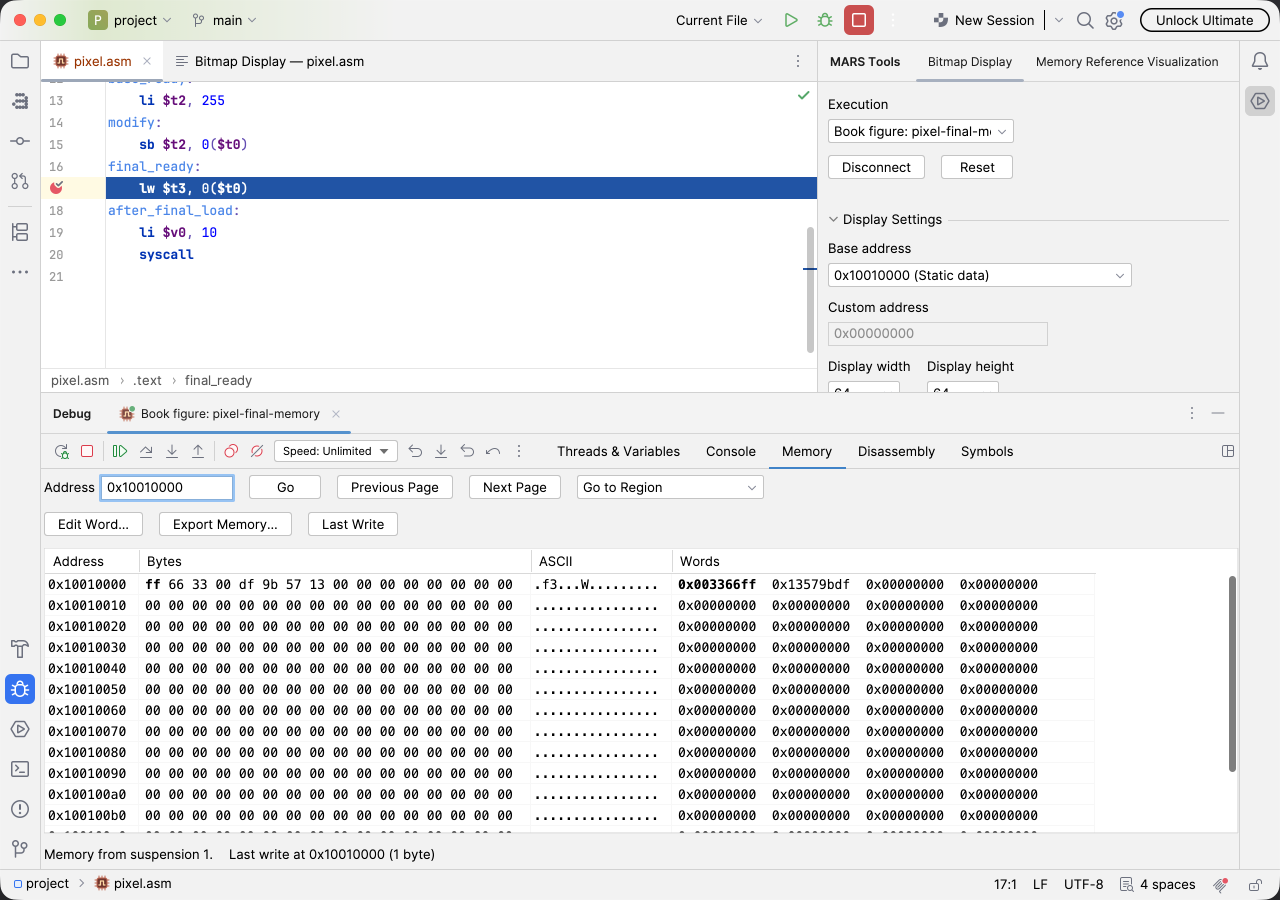
\includegraphics[artifact]{book/captures/002-single-pixel/f02-byte-update/memory.png}}
\sbox2{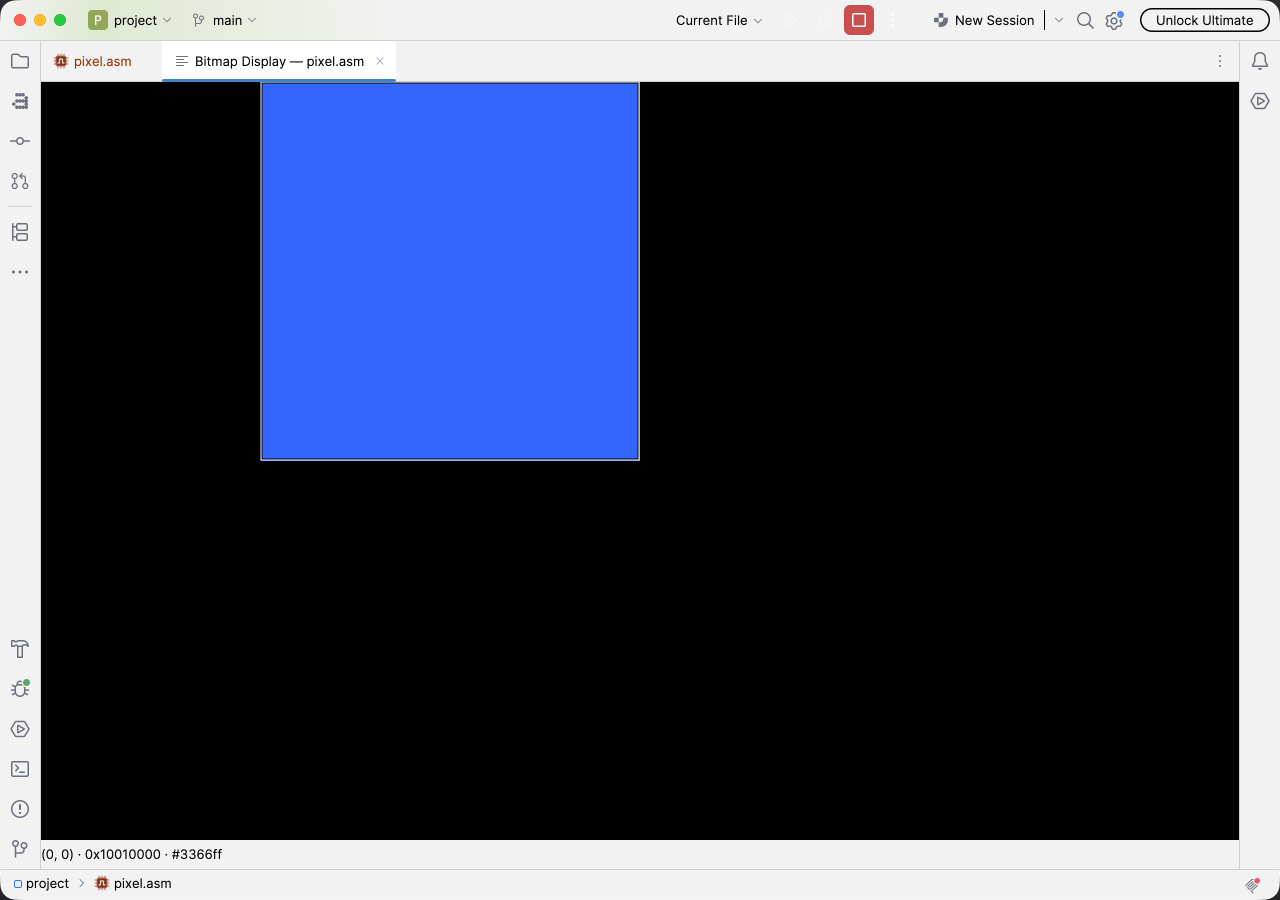
\includegraphics[artifact]{book/captures/002-single-pixel/f02-byte-update/bitmap.png}}
\edef\MARSfinalsourceLeft{\the\dimexpr0.036718750\wd0\relax}
\edef\MARSfinalsourceBottom{\the\dimexpr0.774444444\ht0\relax}
\edef\MARSfinalsourceRight{\the\dimexpr0.611718750\wd0\relax}
\edef\MARSfinalsourceTop{\the\dimexpr0.147777778\ht0\relax}
\edef\MARSfinalmemoryLeft{\the\dimexpr0.034375000\wd0\relax}
\edef\MARSfinalmemoryBottom{\the\dimexpr0.334444444\ht0\relax}
\edef\MARSfinalmemoryRight{\the\dimexpr0.578906250\wd0\relax}
\edef\MARSfinalmemoryTop{\the\dimexpr0.608888889\ht0\relax}
\edef\MARSfinalbitmapLeft{\the\dimexpr0.203906250\wd2\relax}
\edef\MARSfinalbitmapBottom{\the\dimexpr0.066666667\ht2\relax}
\edef\MARSfinalbitmapRight{\the\dimexpr0.203906250\wd2\relax}
\edef\MARSfinalbitmapTop{\the\dimexpr0.091111111\ht2\relax}
\begin{tikzpicture}[alt={Three annotated IDE details at final_ready. The next instruction is lw t3 zero t0, after sb t2 zero t0. The first four memory bytes are ff 66 33 00; the neighbor bytes remain df 9b 57 13. The upper-left display cell is RGB 33 66 ff and the other three cells are black.}]
\node[anchor=north west,inner sep=0,font=\small\bfseries] (source-title) at (6mm,0) {The byte store has executed; the load is next};
\node[anchor=north west,inner sep=0] (source) at ([yshift=-1mm]source-title.south west) {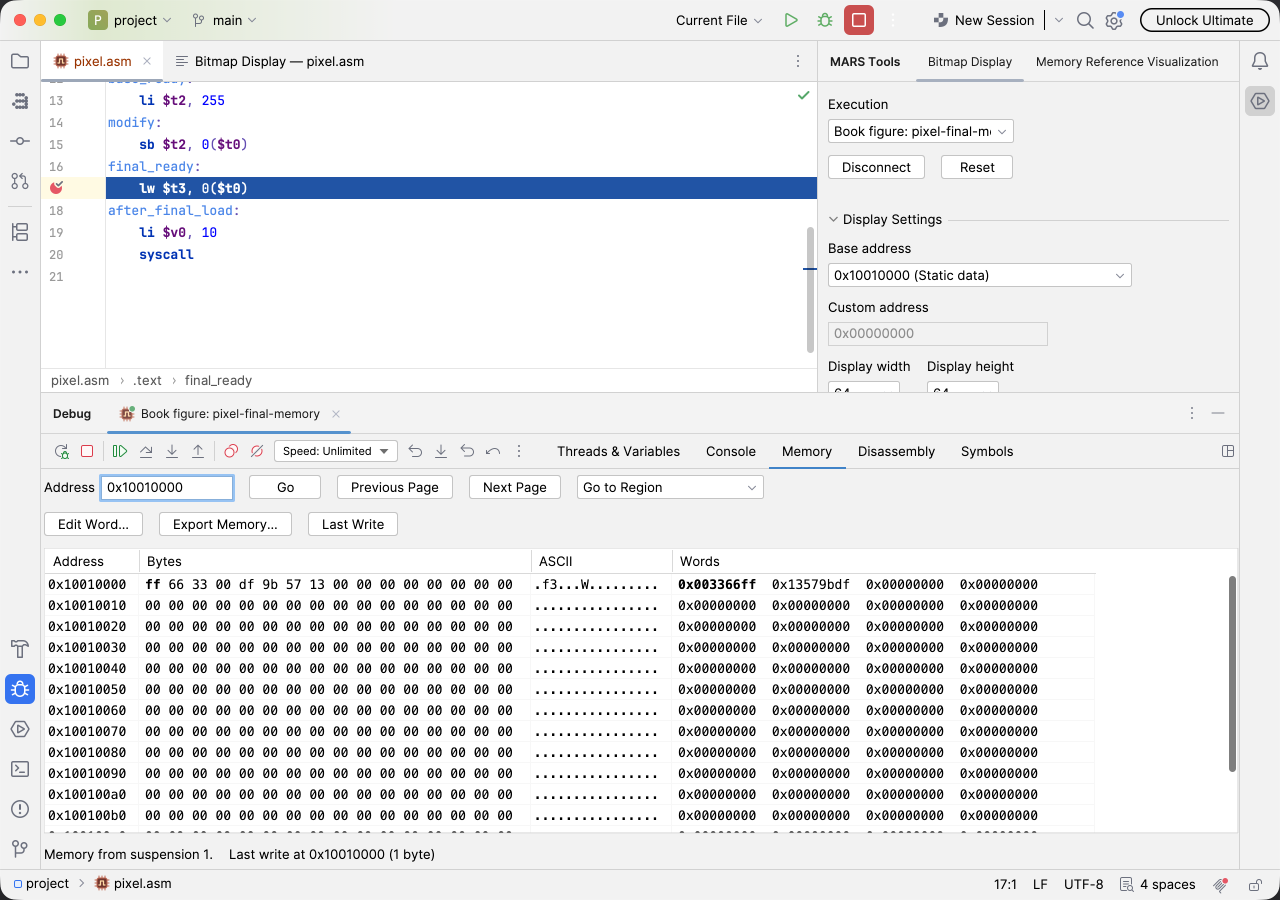
\includegraphics[width=0.7\linewidth,artifact,trim={\MARSfinalsourceLeft{} \MARSfinalsourceBottom{} \MARSfinalsourceRight{} \MARSfinalsourceTop{}},clip]{book/captures/002-single-pixel/f02-byte-update/memory.png}};
\begin{scope}[shift={(source.south west)},x={($(source.south east)-(source.south west)$)},y={($(source.north west)-(source.south west)$)}]
\draw[black,line width=0.7pt] (0.135555556,0.054054054) rectangle (0.446666667,0.351351351);
\node[draw=black,fill=white,circle,inner sep=1.5pt,font=\footnotesize] at ($(0.135555556,0.351351351)+(-3mm,0)$) {1};
\end{scope}
\node[anchor=north west,inner sep=0,font=\small\bfseries] (memory-title) at ([yshift=-2mm]source.south west) {Only the byte at offset zero changed};
\node[anchor=north west,inner sep=0] (memory) at ([yshift=-1mm]memory-title.south west) {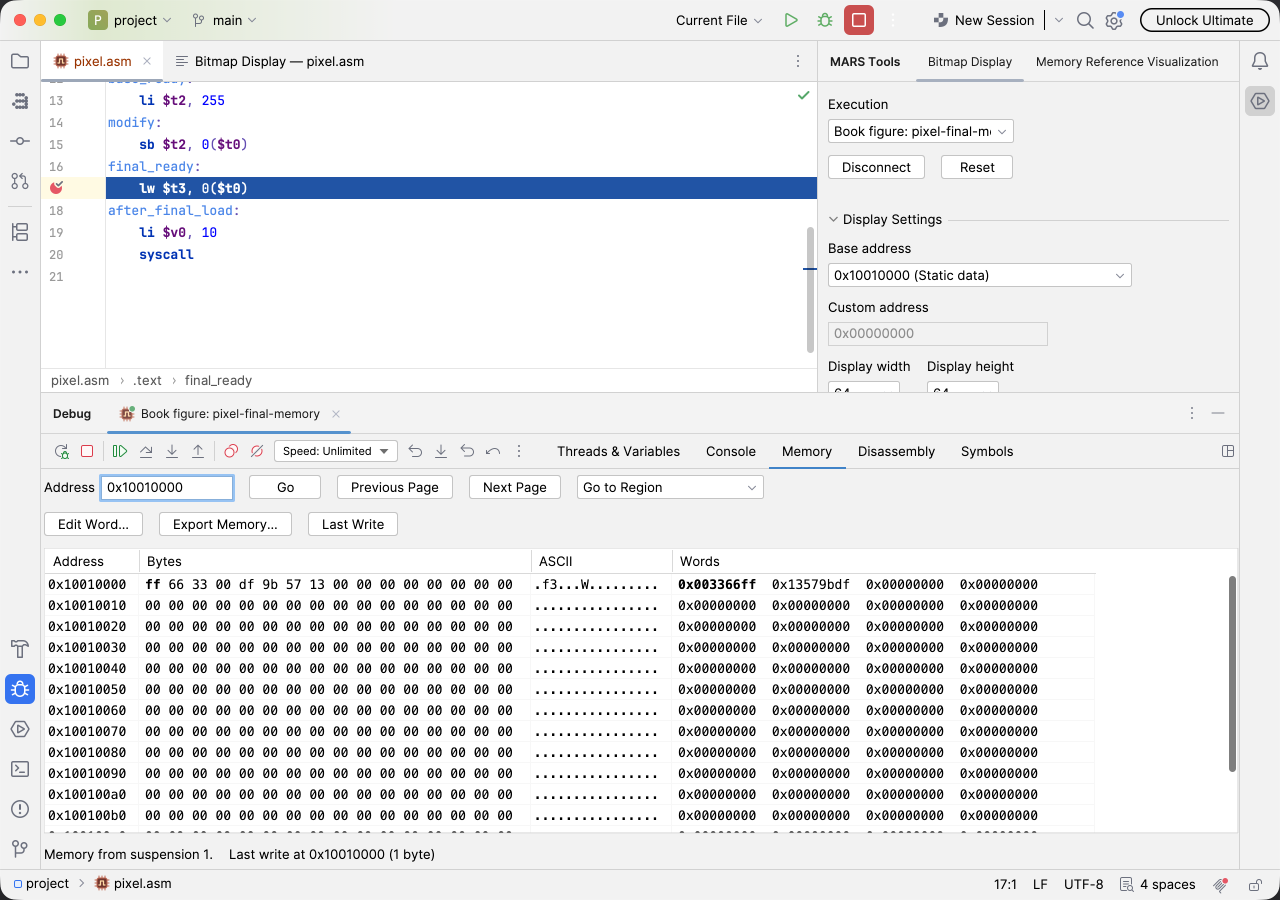
\includegraphics[width=0.84\linewidth,artifact,trim={\MARSfinalmemoryLeft{} \MARSfinalmemoryBottom{} \MARSfinalmemoryRight{} \MARSfinalmemoryTop{}},clip]{book/captures/002-single-pixel/f02-byte-update/memory.png}};
\begin{scope}[shift={(memory.south west)},x={($(memory.south east)-(memory.south west)$)},y={($(memory.north west)-(memory.south west)$)}]
\draw[black,line width=0.7pt] (0.191919192,0.078431373) rectangle (0.983838384,0.490196078);
\node[draw=black,fill=white,circle,inner sep=1.5pt,font=\footnotesize] at ($(0.191919192,0.490196078)+(-3mm,0)$) {2};
\end{scope}
\node[anchor=north west,inner sep=0,font=\small\bfseries] (bitmap-title) at ([yshift=-2mm]memory.south west) {The display reads the updated packed word};
\node[anchor=north west,inner sep=0] (bitmap) at ([yshift=-1mm]bitmap-title.south west) {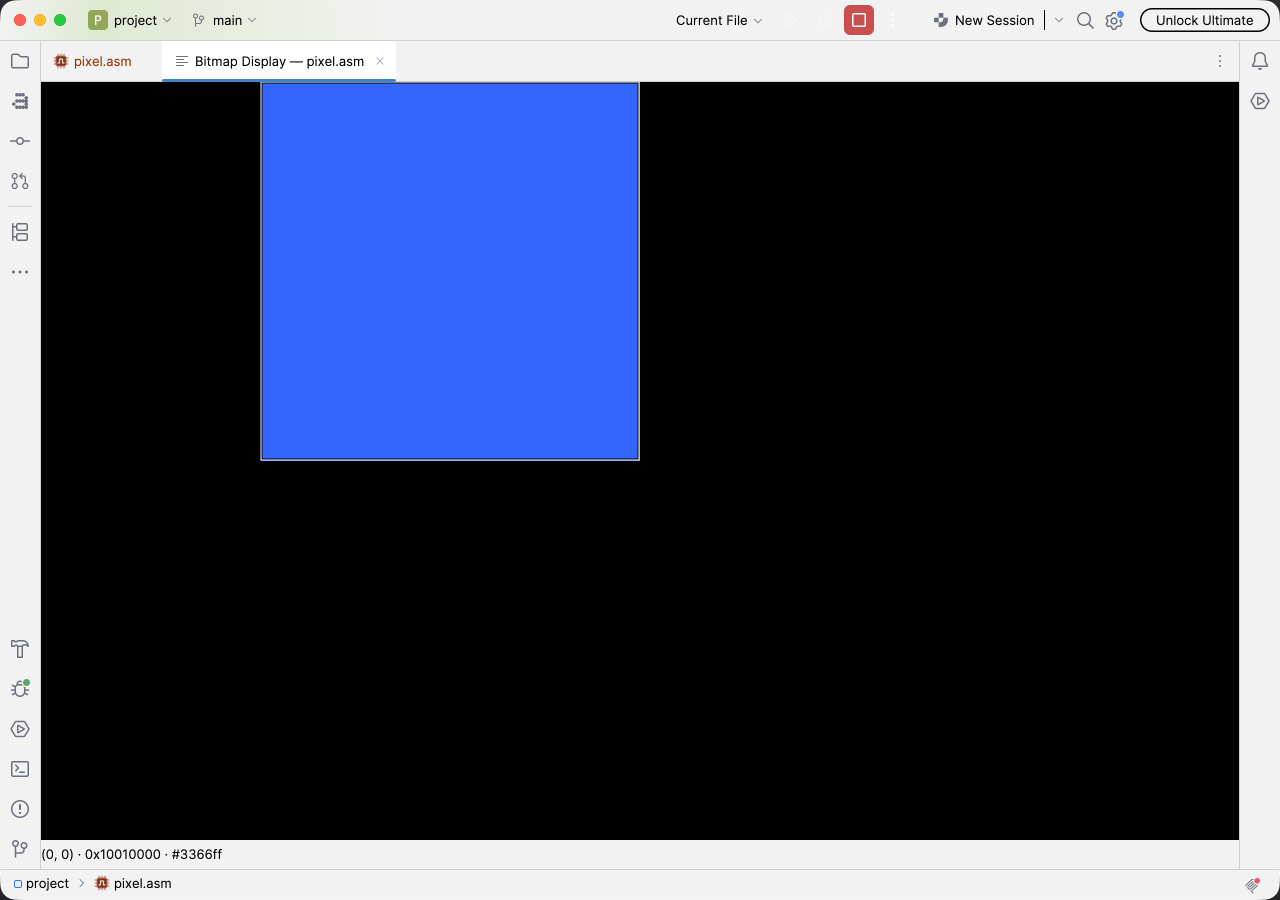
\includegraphics[width=0.32\linewidth,artifact,trim={\MARSfinalbitmapLeft{} \MARSfinalbitmapBottom{} \MARSfinalbitmapRight{} \MARSfinalbitmapTop{}},clip]{book/captures/002-single-pixel/f02-byte-update/bitmap.png}};
\begin{scope}[shift={(bitmap.south west)},x={($(bitmap.south east)-(bitmap.south west)$)},y={($(bitmap.north west)-(bitmap.south west)$)}]
\draw[black,line width=0.7pt] (0.000000000,0.000000000) rectangle (1.000000000,1.000000000);
\node[draw=black,fill=white,circle,inner sep=1.5pt,font=\footnotesize] at ($(0.000000000,1.000000000)+(-3mm,0)$) {3};
\end{scope}
\end{tikzpicture}
\par\smallskip
\begin{minipage}{\linewidth}
\small
\begin{enumerate}
\item The completed \texttt{sb \$t2, 0(\$t0)} wrote the low eight bits of 255 at offset zero. The highlighted \texttt{lw \$t3, 0(\$t0)} has not executed. Do not use \texttt{\$t3} as the readback result yet.
\item The bytes are now \texttt{ff 66 33 00}, representing \texttt{0x003366ff}. Only \texttt{99} became \texttt{ff}. The following neighbor remains \texttt{df 9b 57 13}; the eight trailing zero bytes lie beyond both words.
\item The blue field has increased from \texttt{99} to \texttt{ff}, or 255. Red and green remain \texttt{33} and \texttt{66}. Bitmap Display rereads the containing word after the byte write, so it continues to display a complete RGB color.
\end{enumerate}
\end{minipage}
\caption{After \texttt{sb} changes one byte, before \texttt{lw} reads the word back. Two native Debug views share the stop before the word load.}
\label{capture:002-single-pixel-f02-byte-update}
\end{figure}
